
\graphicspath{ {\curdir/Graphics/}  }

The motional states of trapped ions are shared between all ions in the trap and provide a mechanism for transferring information between these ions.  By applying detuned lasers, virtual phonons can be excited and absorbed in motional modes shared by two or more ions, and the entangling M\o{}lmer-S\o{}rensen gate can be implemented.  In order for this to work the modes must be kept relatively cold, using Doppler cooling or other techniques.  For chains that include mixed ion species, the normal modes can separate, with some modes only coupling to one ion species and some to the other.  This effect limits our ability to cool both ion species using only cooling lasers addressing one species.  We have begun investigating the ion temperatures and heating rates in mixed species chains.  For the moment, we are performing these measurements in a standard macroscopic linear rf trap, but we plan to begin using them to characterize different surface trap designs in the near future.

\section{Single Ion Normal Modes}
\label{sec:single-modes}

In the case of a single ion occupying a trapping region there are only three normal modes.  At the bottom of the trap, the ion sees a harmonic potential in each direction and its motional states are well described by quantum harmonic oscillator states.  We will begin by only considering one mode of motion in the $\hat{x}$ direction.  We can label the motional states by $\ket{0}$, $\ket{1}$, etc. with energy $E_n = \hbar \omega (n + \frac{1}{2})$.  We can also define raising and lowering operators $a$ and $a^\dagger$ and write the position of the ion in terms of them as $x = x_0 (a + a^\dagger)$ where $x_0 = \sqrt{\frac{\hbar}{2 m \omega_x}}$ and $m$ is the mass of the ion.  After Doppler cooling the ion is in a thermal mixed state of these motional levels.  The density matrix of the ion is described by a parameter $\bar{n}$, the average thermal motional occupation number, and can be written
\begin{equation}
	\rho = \sum\limits_{n=0}^{\infty} \frac{1}{\bar{n}+1} \left( \frac{\bar{n}}{\bar{n} + 1} \right) ^ n \ket{n} \bra{n} \mathrm{.}
\end{equation}

In order to analyze the temperature of the motional modes we first took some measurements with a single ion.  In particular, we measured $\bar{n}$ and its time derivative $\dot{\bar{n}}$ to determine these parameters in the linear rf trap where we will later perform mixed ion species experiments.  The initial average thermal motional occupation number, $\bar{n}$, provides information on how effective Doppler cooling is, and can be indicative of problems with the cooling laser powers and frequencies.  The parameter $\dot{\bar{n}}$ is often called the heating rate, and is likely to be roughly constant as more ions are added.  Heating rates in macroscopic traps are often less problematic than in surface traps because of the increased distance between the nearest surfaces and the trapping locations, but the techniques we develop can later be used when these experiments are moved to surface traps.  

In order to make measurements of these parameters of the normal modes of the ion trap, we have to understand the way electric fields can interact with the modes.  In particular, we will be driving sideband transitions using lasers addressing narrow optical transitions.  Consider an atomic system consisting of two qubit levels $\ket{\downarrow}$ and $\ket{\uparrow}$, as well as harmonic motional energy levels in the $\hat{x}$ direction with angular frequency $\omega_x$.  Our base Hamiltonian is then
\begin{equation}
	H = \hbar \omega_\downarrow \ket{\downarrow}\bra{\downarrow} + \hbar \omega_\uparrow \ket{\uparrow}\bra{\uparrow} + \hbar \omega_x a^\dagger a \mathrm{,}
\end{equation}
where $\hbar \omega_\downarrow$ and $\hbar \omega_\downarrow$ are the energies of the two qubit levels.  We will consider the interaction of this ion with monochromatic electromagnetic radiation described by the potential energy
\begin{equation}
	V = \hbar \Omega \left( \ket{\uparrow}\bra{\downarrow} + \ket{\downarrow} \bra{\uparrow} \right) \left( e^{i k_x x + i \omega t} + h.c. \right) \mathrm{,}
\end{equation}
where $k_x$ is the component of the photon wavevector in the $\hat{x}$ direction, $\omega$ is the angular frequency of the radiation, $\Omega \equiv \frac{\vec{\mu} \cdot \vec{E}}{\hbar}$ is the Rabi frequency of the transition defined as in Chapter~\ref{sec:qcomp} in terms of the electric field magnitude and polarization, $\vec{E}$, and the ion dipole moment, $\vec{\mu}$.  Transforming the Hamiltonian into the interaction picture, we find
\begin{equation}
	V_I(t) = \hbar \Omega \left( \ket{\uparrow}\bra{\downarrow} \exp \left( i \eta (a e^{-i \omega_x t} + a^\dagger e^{i \omega_x t}) + i (\omega - \omega_{\uparrow} + \omega{\downarrow}) t \right) + h.c. \right) \mathrm{,}
\end{equation}
where $\eta \equiv x_0 k_x$ is the Lamb-Dicke parameter defined in Chapter~\ref{sec:qcomp}.  The effect of the ion's motion on the optical transitions between motional states $n$ and $n'$ can be absorbed into $\Omega$ and $\delta$ by writing
\begin{eqnarray}
	\Omega_{n,n'} &=& \Omega \left| \bra{n'} \exp\left( i \eta (a + a^\dagger ) \right) \ket{n} \right| \\
	&=& \Omega e^{-\eta^2 / 2} \left( \frac{n_<!}{n_>!} \right)^{1/2} \eta^{\left| n - n' \right| } L_{n_<}^{\left| n - n' \right| }(\eta^2) \\
	\delta_{n,n'} &=& \omega - \omega_\uparrow + \omega_\downarrow - \omega_x (n' - n)
\end{eqnarray}
using the generalized Laguerre polynomials, $L_n^\alpha$, and defining the smaller of $n$ and $n'$ to be $n_<$ and the larger to be $n_>$.  The transition between $\ket{\uparrow}$ and $\ket{\downarrow}$ proceeds as in Chapter~\ref{sec:qcomp}, but with additional transitions corresponding to any choice of $n$ and $n'$ occurring with the corresponding $\Omega_{n,n'}$ and $\delta_{n,n'}$.

Therefore, we can see that we can drive transitions between motional states of the ion using an optical electric field.  In order to observe these sideband transitions in trapped barium ions, we use the techniques discussed in Section~\ref{sec:initread}.  We trap and Doppler cool a single \ba ion, and then initialize its state to the $m_J$ = -1/2 level of its 6S$_{1/2}$ ground state by switching our cooling laser to have circular polarization.  We then shutter the cooling lasers and apply a fixed duration pulse of 1762~nm light that is near the transition from the optically pumped ground state to the $m_J$ = -1/2 level of the 5D$_{5/2}$ state.  Upon reactivating the cooling lasers we see fluorescence from the ion only if we were unsuccessful in driving a transition with 1762~nm laser.  This procedure is repeated multiple times to build statistics, and then repeated at multiple frequencies of the 1762~nm laser to explore the frequency dependence of the transition. 

Figure~\ref{fig:freqscan} shows the result of this procedure.  The large center peak is the carrier transition ($n'$ = $n$) that does not include any change in motional state.  There are two sets of red ($n'$ = $n-1$) and blue ($n'$ = $n+1$) sidebands of this transition visible corresponding to the two radial motional modes.  The strength of the sidebands is related to the carrier transition by $\eta \sqrt{\bar{n}}$ and therefore depends on the photon momentum, the motional secular frequency, and the occupation number.  The two sidebands that are shown are the radial sidebands with secular frequencies of $\omega_x$ = $2 \pi \times$ 1.31~MHz and $\omega_y$ = $2 \pi \times$ 1.21~MHz.  The 1762~nm laser is oriented perpendicular to the trap axis and therefore no axial sideband transition can be seen because the corresponding $\eta = 0$.

\begin{figure}
	\centering
	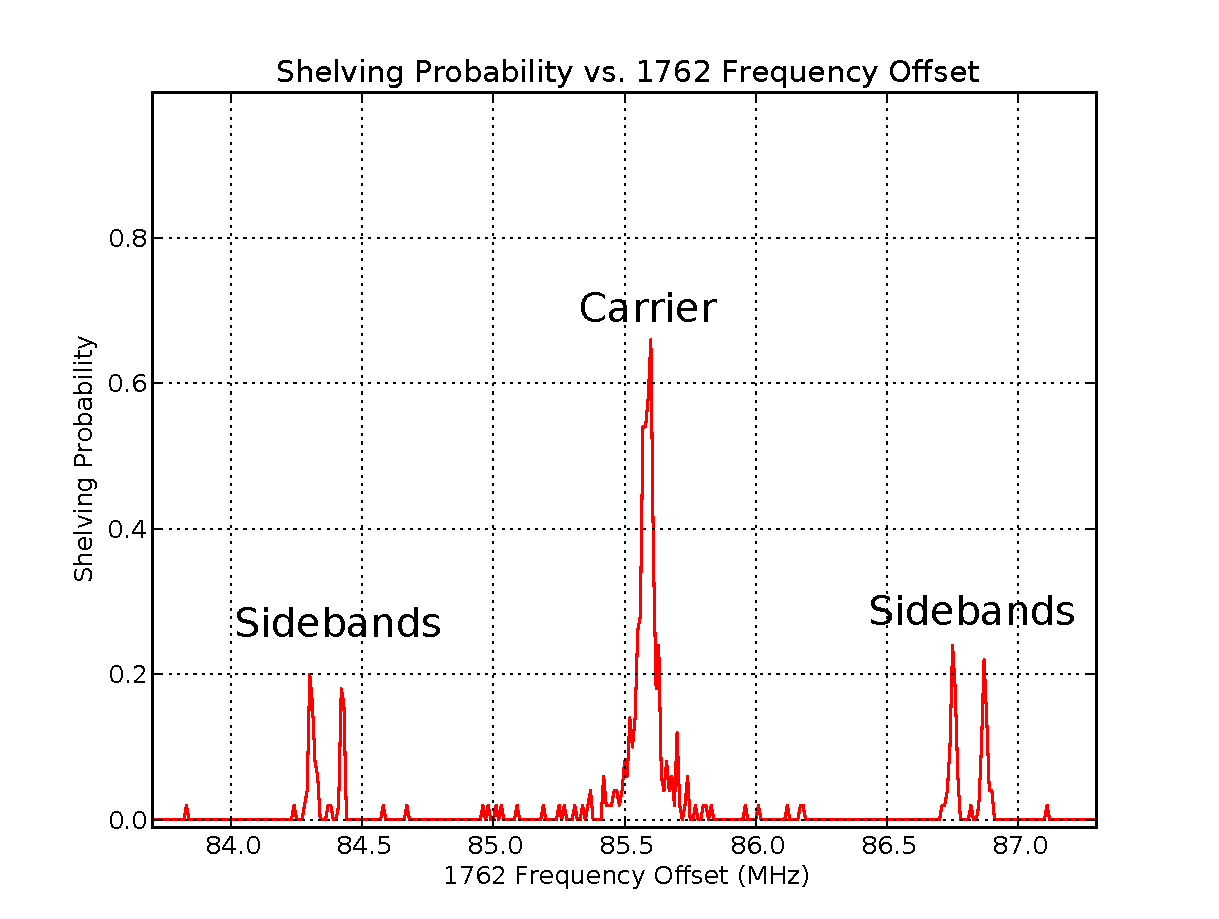
\includegraphics[width=0.8\textwidth]{FullScan}
\caption[Motional mode spectroscopy of the 1762~nm transition in \ba]{Motional mode spectroscopy of the 1762~nm transition in \ba.  Shelving probability is shown as a function of 1762~nm laser frequency.  A strong carrier transition is present at offset 85.6~MHz, while symmetric radial motional sidebands can be seen at 84.3~MHz, 84.4~MHz, 86.75~MHz, and 86.85~MHz.}
	\label{fig:freqscan}
\end{figure}

Using this technology we would then like to estimate the initial temperature and heating rate of our ions.  There are two possible methods for performing this procedure.  We could compare the strength of the sidebands to the strength of the carrier and use the weak excitation limit from Equation~\ref{eqn:shortpulses} to extract $\eta \sqrt{\bar{n}}$ for each peak.  The difficulty with this strategy is that the radial modes must be weakly excited in order to extract this information, and errors on fitting the heights of the peaks are often large.  For single ions we can make a more accurate measurement by using a different technique based on measuring the decay of contrast in carrier Rabi oscillations.

Since our 1762~nm source has a linewidth $<$ 1~kHz we should be able to apply pulses of hundreds of microseconds of duration without seeing any noticeable loss of contrast in Rabi oscillations.  Instead the amplitude of these oscillations begins to decay in 100~$\mu$s to 200~$\mu$s because of the finite temperature of our ions.  The source of this loss of contrast is driving carrier (not sideband) transitions from different motional harmonic oscillator states.  The sideband transitions are far enough away in frequency that they are not relevant, but these carrier transitions at different motional energies are slightly shifted in frequency with respect to one another.  All of these transitions of slightly different frequency are driven simultaneously and the accumulating phase difference between them causes a decrease in contrast.

The Rabi frequency for these carrier transitions follows from the above discussion of sideband transitions and is
\begin{equation}
	\Omega_{n,n} = \Omega e^{-\eta^2/2} L_n^0 ( \eta^2 ) \mathrm{,}
\end{equation}
which can be simplified for $\eta^2 \ll 1$ to $\Omega ( 1 - \eta^2 n )$.  In order to calculate the result for an ion at a finite temperature we can write the probability of driving the transition as a sum over a thermal distribution of motional states. The probability of driving the transition to the shelved state becomes
\begin{equation}
P_\mathrm{shelve} (t) = \sum\limits_{n=0}^{\infty} \frac{1}{\bar{n} + 1} \left( \frac{\bar{n}}{\bar{n} + 1} \right) ^n \sin^2 \left( \Omega_{n,n}  \frac{t}{2} \right) 
\end{equation}
This analysis has all been performed assuming there is only one motional degree of freedom.  If the ion has multiple modes of motion there is a corresponding Lamb-Dicke parameter, $\eta$, and thermal average occupation number, $\bar{n}$, for each mode.  The shelving probability can be calculated by summing over all possible combinations of occupation numbers in each mode weighted by the thermal state probability for each mode.  For even a few modes this calculation becomes very time consuming, and the fit parameters are coupled together which decreases the accuracy of the fit.  The computational time can be reduced by Monte Carlo sampling from the distribution of occupation numbers, but the errors would still be large.

Instead we have chosen the propagation angle of the 1762~nm laser to only address the radial modes of motion, which are separated in frequency by $\le$ 10\%.  It is therefore reasonable to approximate their occupation numbers and Lamb-Dicke parameters as equal.  Since the axial trap frequency is almost an order of magnitude smaller this procedure would not be possible if the 1762~nm laser also addressed these states.  Making this approximation for the radial parameters, we can extract a parameter $\sum_i \bar{n}_i$, where the sum extends over two radial modes, from an experimental Rabi flop curve.

Using this procedure, we would like to find the minimum temperature we achieve with Doppler cooling, as well as the rate at which the ion heats while Doppler cooling is disabled.  In order to find this heating rate, we can shutter the cooling lasers for a variable period of time before applying 1762~nm pulses to it.  In Figure~\ref{fig:rabi-heating} we can see that as we increase the period of time that the cooling lasers are shuttered the Rabi oscillations lose contrast more rapidly which corresponds to an increase in temperature of the ion.  It is common to approximate the heating rate in ion traps as linear, and this approximation holds well at least for low temperatures.  As the ion heats up and experiences more of the trap anharmonicity and trap micromotion, heating rates may increase, but we do not see evidence of this at the temperatures we currently reach.  The total initial radial mode average occupation of our single trapped barium ion is 122~quanta for two modes, with a total heating rate of 2.43~quanta/ms (see Figure~\ref{fig:heating-nonoise}).

\begin{figure}
	\centering
	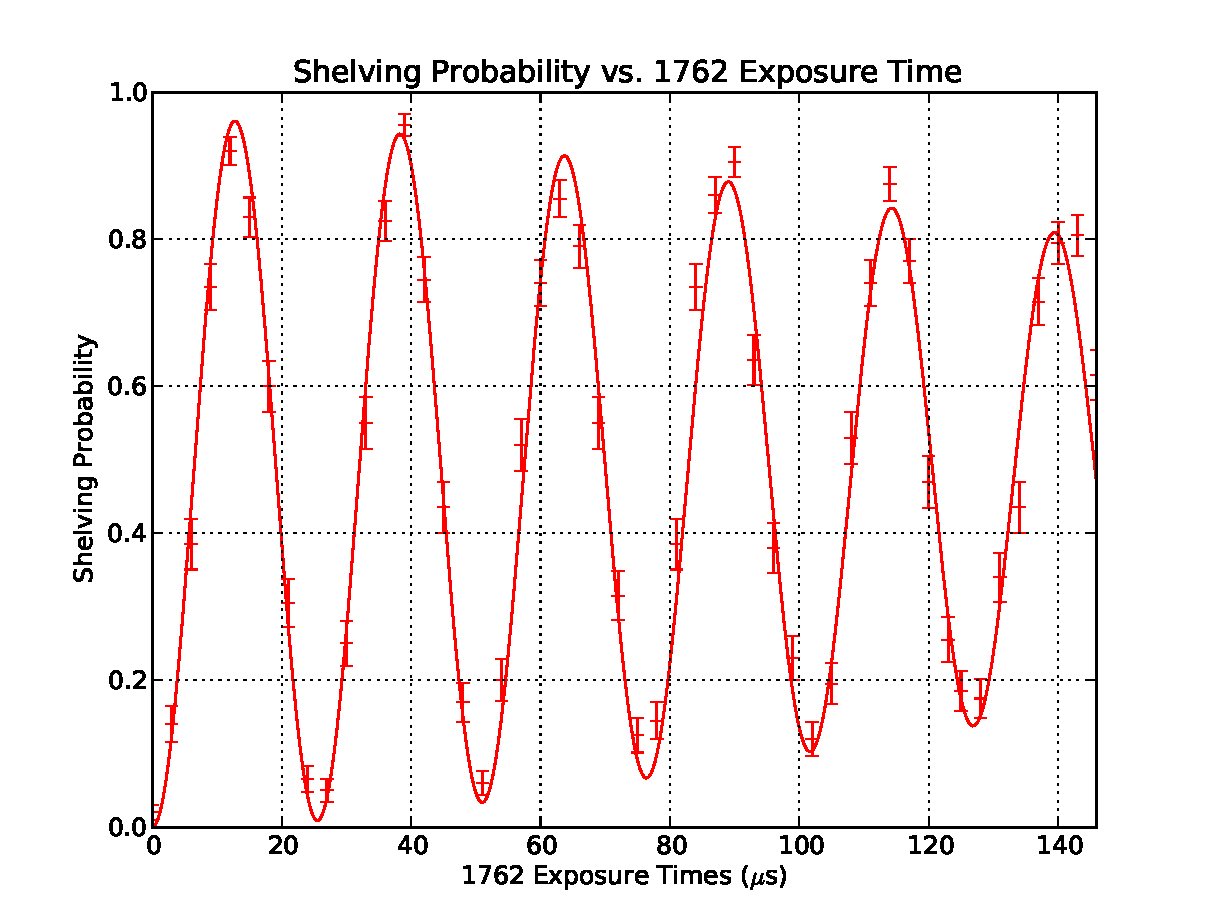
\includegraphics[width=0.7\textwidth]{HeatingRateT0Orange}
	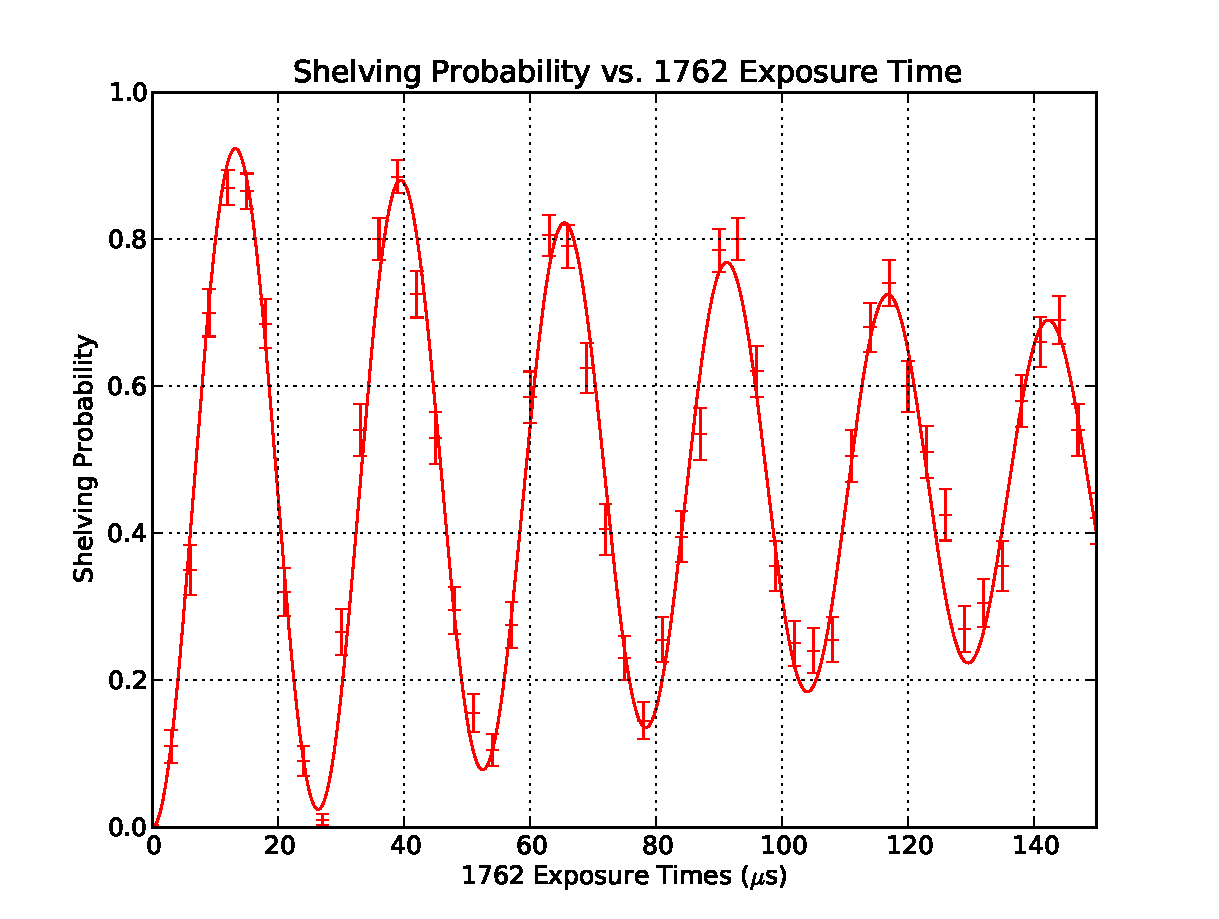
\includegraphics[width=0.7\textwidth]{HeatingRateT50000Orange}
	\caption[Rabi oscillations on the 1762~nm transition at different ion temperatures]{Rabi oscillations with different delays between the end of Doppler cooling and the beginning of 1762~nm laser exposure.  The contrast of the Rabi oscillations decays more quickly after a delay of 50~ms (bottom) than with no delay (top).}
	\label{fig:rabi-heating}
\end{figure}


\begin{figure}
	\centering
	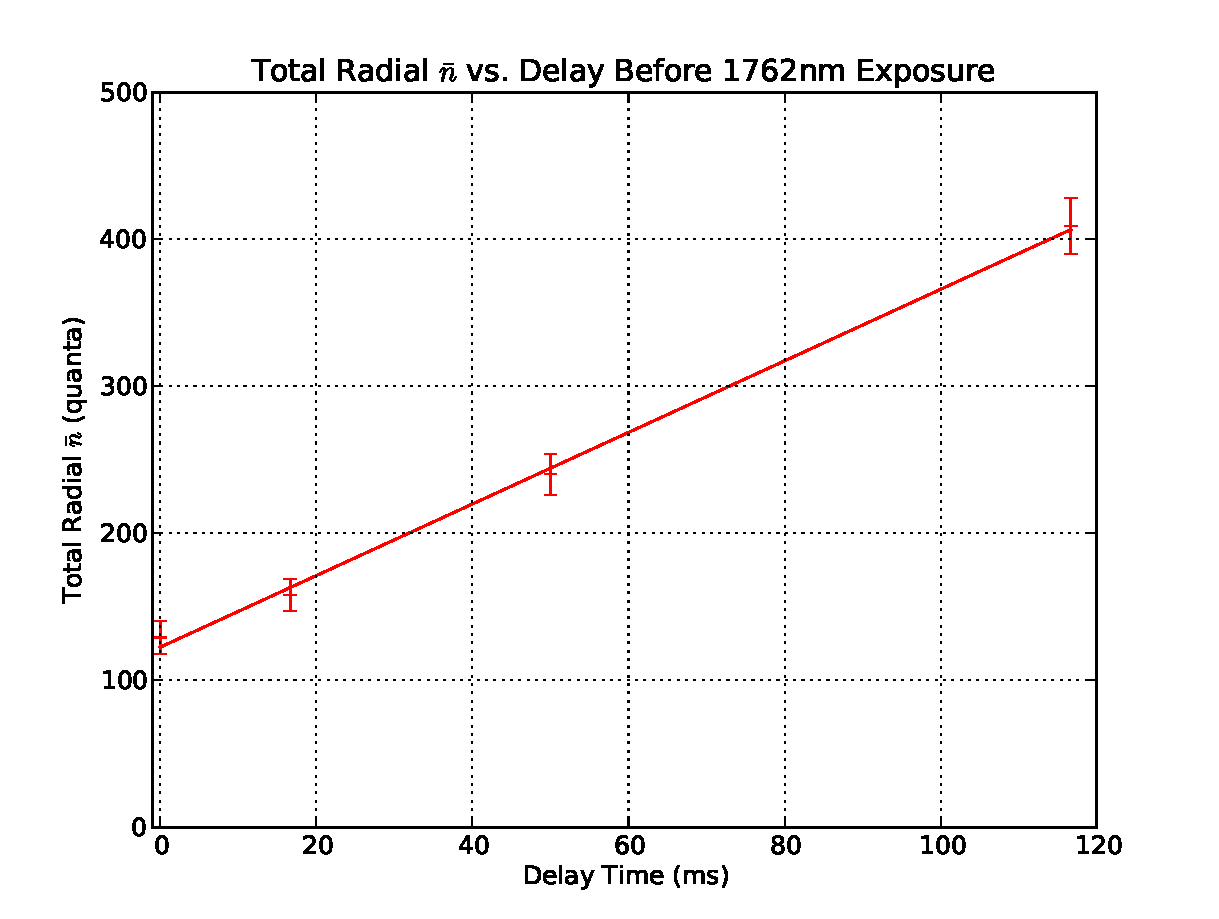
\includegraphics[width=0.8\textwidth]{HeatingRate}
	\caption[Heating rate of single barium ion without 1762~nm noise correction]{Heating rate of a single barium ion without correcting for 1762~nm frequency noise.  Total thermal radial mode average occupation number is plotted as a function of delay time during which the ion is not cooled.  A linear fit is shown with initial total radial average thermal occupation number of 122~quanta and a 2.43~quanta/ms heating rate.}
	\label{fig:heating-nonoise}
\end{figure}

Unfortunately, the initial temperature of the ion that we measured with this procedure was significantly hotter than expected.  Doppler cooling barium ions with 493~nm light should result in ion temperatures of $<$ 0.5~mK from Equation~\ref{eqn:doppler}. The measured initial temperature is approximately an order of magnitude higher at $\approx$ 60 quanta per radial mode of motion, which corresponds to $\approx$ 3.5~mK.  By carefully exploring the dependence of the decay of our Rabi oscillations with temperature we determined that our initial ion temperature is not actually this large.  Instead, there is an increased loss of contrast caused by frequency variations in our 1762~nm laser.

This laser is locked to a 500~kHz linewidth cavity by a locking circuit that stabilizes it to within a few percent of the cavity linewidth.  The small residual error still corresponds to a frequency modulation of the laser with a modulation depth of 10~kHz, but the timescale of the modulation is very slow compared to the duration of the pulses we apply to the ion.  The result is that every run of our Rabi flop experiment sees an approximately constant frequency drawn from this 10~kHz wide distribution of frequencies.  By sampling from this distribution in the fit function we can correct the measured Doppler temperature for this additional effect.  The shelving probability, $P_{\mathrm{shelved}}$, is then given by
\begin{eqnarray}
	P_\mathrm{shelved}(t) &=& \int_\omega \frac{1}{\sigma \sqrt{2 \pi}} e^{-\frac{(\omega - \mu)^2 }{2 \sigma^2}} \sum\limits_{n=0}^\infty \frac{1}{\bar{n} + 1} \left( \frac{\bar{n}}{\bar{n} + 1} \right)^2 \frac{s \Omega^2}{W^2} \sin^2 \left( W (1 - \eta^2 n) \frac{t}{2} \right) \\
	W(\omega)^2 &\equiv& \Omega^2 + (\omega - \omega_\mathrm{transition})^2
\end{eqnarray}
where $\sigma$ is the width of the residual frequency noise ($\approx$ 10~kHz), $\mu$ is the center frequency of this distribution which is approximately equal to $\omega_\mathrm{transition}$ which is the center of the 1762~nm transition, and $\Omega$ is the Rabi frequency ($\approx$ 50~kHz with our achievable laser power).  The resulting curve also exhibits a loss of contrast on the 100~$\mu$s time scale.

The fit parameters are the Rabi frequency $\Omega$, the optical pumping efficiency $s$, and the sum of the radial average thermal occupation numbers $\sum_i \bar{n}_i$.  In Figure~\ref{fig:heating} we have fit this new model to the same data and the heating rate of the radial modes is again approximately linear, with an initial temperature that is reasonable for a Doppler cooled barium ion.  The linear fit shown corresponds to an initial $\sum_i \bar{n}_i$ = 17~quanta, with a heating rate of 2.84~quanta/ms.  The corresponding minimum Doppler temperature is $\approx$ 1~mK, which agrees reasonably well with the theoretical minimum given the saturation of the 493~nm transition and the complicating effect of the 650~nm repump laser.  We will use these single ion measurements to evaluate our results with ion chains in the next section.  We expect that the heating rate per ion should be approximately constant.

\begin{figure}
	\centering
	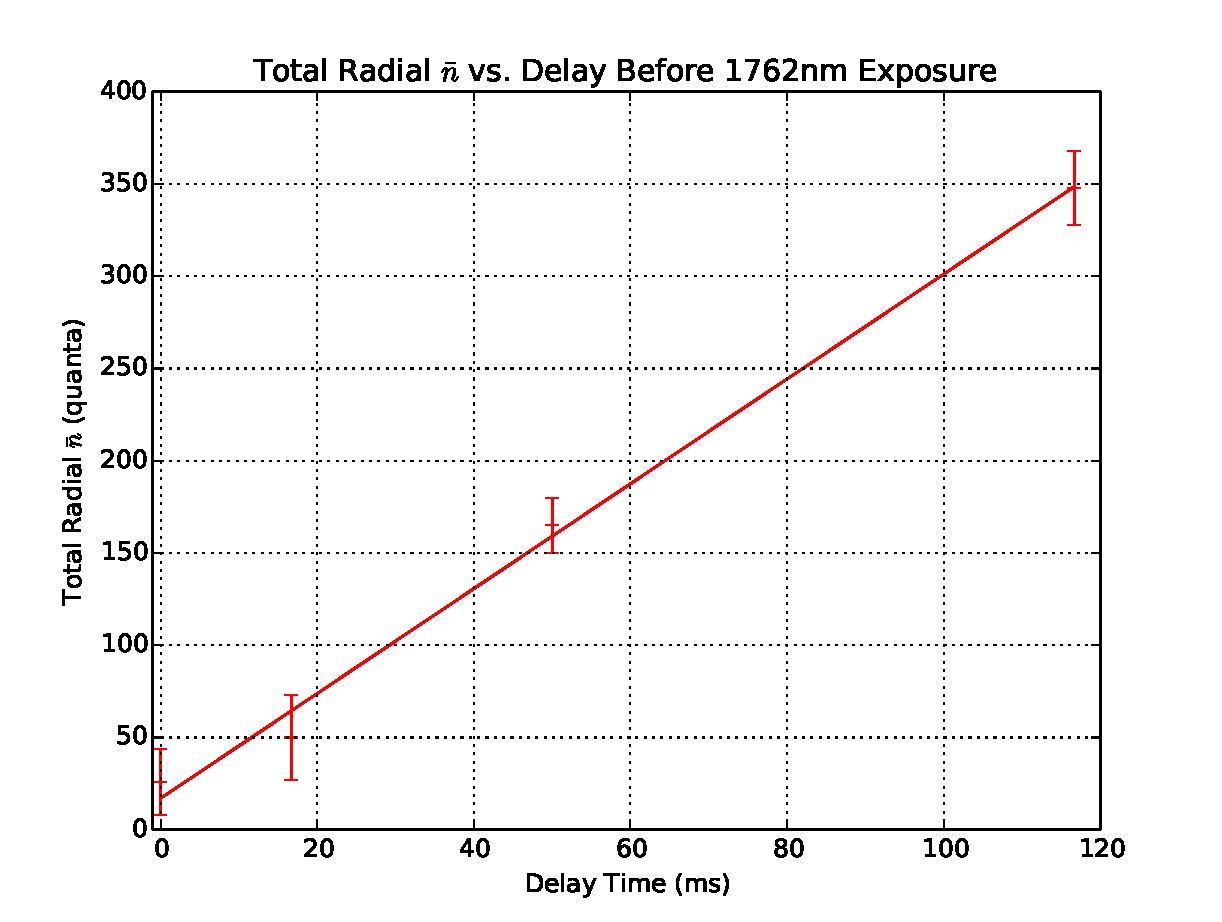
\includegraphics[width=0.8\textwidth]{HeatingRateNoise}
	\caption[Heating rate of single barium ion]{Heating rate of a single barium ion in a linear rf trap.  Measured radial motional average occupation numbers as a function of the period of time the ion was allowed to heat before the 1762~nm pulse began.  A linear fit is shown with initial radial average thermal occupation number of 17~quanta and a 2.84~quanta/ms heating rate.}
	\label{fig:heating}
\end{figure}

\section{Mixed Species Ion Chains}
\label{sec:mixed-modes}

In order to analyze the temperatures of mixed species chains, we first need to understand the normal mode structure of a chain of ions with different masses.  The normal modes for any given number of each species of ion and any ordering of those species can be calculated through classical mechanics techniques.  When the dynamics are much slower than the rf period, the Mathieu equation can be ignored and the trapping potential can be written as a simple harmonic oscillator.  The trapping potential is then
\begin{equation}
	V_\mathrm{trap} = \sum\limits_{i=1}^N \frac{1}{2} m_i \omega_x^2(m_i) x^2 + \frac{1}{2} m_i \omega_y^2(m_i) y^2 + \frac{1}{2} m_i \omega_z^2(m_i) z^2 \mathrm{,}
\end{equation}
where $N$ is the number of ions in the trap, $m_i$ is the mass of ion $i$, and $\omega_z$ is the axial confinement generated by the dc electrodes that is necessarily weaker than the radial secular frequencies $\omega_x$ and $\omega_y$.  The trap frequencies are a function of the ion mass as described in Equations~\ref{eqn:axialfreq} and \ref{eqn:radialfreq}.  The trap potential is modified by the Coulomb interaction between the ions
\begin{equation}
	V_\mathrm{coulomb} = \frac{1}{2} \sum\limits_{i = 1}^N \sum\limits_{j \ne i} \frac{1}{4 \pi \epsilon_0} \frac{q^2}{ \left| \vec{x}_i - \vec{x}_j \right| } \mathrm{,}
\end{equation}
where $q$ is the charge of an ion.

At the minimum of the potential, the linear terms are zero and the potential can be approximated by
\begin{eqnarray}
	V &=& \sum\limits_{i=1}^{3N} \sum\limits_{j=1}^{3N} V_{ij} x_i x_j \\
	\label{eqn:mixedtrap}
	V_{ij} &\equiv& \frac{1}{\sqrt{m_i m_j}} \frac{ \partial }{ \partial x_i } \frac{ \partial }{ \partial x_j } ( V_\mathrm{trap} + V_\mathrm{coulomb} ) 
\end{eqnarray}
where we have neglected a constant offset and allowed $i$ and $j$ to represent the $\hat{x}$, $\hat{y}$, or $\hat{z}$ direction of any one of the N ions.  Anharmonic terms can be taken into account by evaluating higher derivative tensors and using perturbation theory \cite{Home:11}.  The equations of motion for the harmonic terms are given by
\begin{equation}
	\ddot{x_i} + V_{ij} x_j = 0 \mathrm{.}
\end{equation}
There are 3N solutions which take the form of independent harmonic oscillators.  Each harmonic oscillator corresponds to motion along one of the eigenvectors of the matrix $V_{ij}$ with an angular frequency $\omega_\alpha$ equal to the square root of the corresponding eigenvalue.  We can write these solutions as
\begin{equation}
	\vec{x}_{\alpha}(t) = \hat{e}_{\alpha} \cos(\omega_\alpha t)
\end{equation}
for each normal mode $\alpha$, where $\hat{e}_\alpha$ is a unit length eigenvector of $V_{ij}$.  The analysis of sideband transitions still carries through with one small modification.  The separate motional state operators for each ion and each mode now carry the corresponding eigenvector component as a scalar multiplier that reduces the motion of each individual ion.  This effect can be accounted for by defining our Lamb-Dicke parameter for each mode $\alpha$ and ion $i$ to be $\eta_{\alpha, i} = \hat{e}_{\alpha}^i x_{\alpha, 0} k_x$, where $x_{\alpha, 0} = \sqrt{ \frac{\hbar}{2 m \omega_\alpha} }$.

We can scan the frequency of the 1762~nm laser over these radial modes following almost the same procedure used for a single barium ion.  One difference is that state detection must be done with our EMCCD camera instead of with the PMT.  The PMT has no spatial sensitivity and cannot distinguish which ions in the chain are bright.  Since we need to independently build statistics of each ion's state, we must be able to distinguish which ions are shelves in each experimental run.  I have developed software that integrates our experiment with the EMCCD camera and automatically performs this analysis.

An additional difference is that data must be collected when the ions are ordered in a particular configuration.  The normal mode structure changes depending on the ordering of the ion species and the numbers of each ion.  This structure must be constant in each experimental run.  In the future, this work can be done in microfabricated traps where dc control voltages can be used to separate, reorder, and merge ions.  At the moment, the ions are randomly reordered by shuttering the Doppler cooling lasers and allowing the ions to heat until the ion crystal melts.  When the ions recrystallize their order randomly changes.  This procedure must be repeated until the desired order is achieved at random.   It becomes more unlikely to reach the correct configuration as the number of possible configurations increases which is the current limiting factor in the number of ions we can use in these experiments.

We have performed initial characterizations of chains of two barium and two ytterbium ions.  This chain length is short enough that we can achieve the desired ion ordering easily enough to take reasonable amounts of data.  We are most interested in how effectively the ytterbium ions can be kept cooled by only Doppler cooling the barium ions.

\begin{figure}
	\centering
	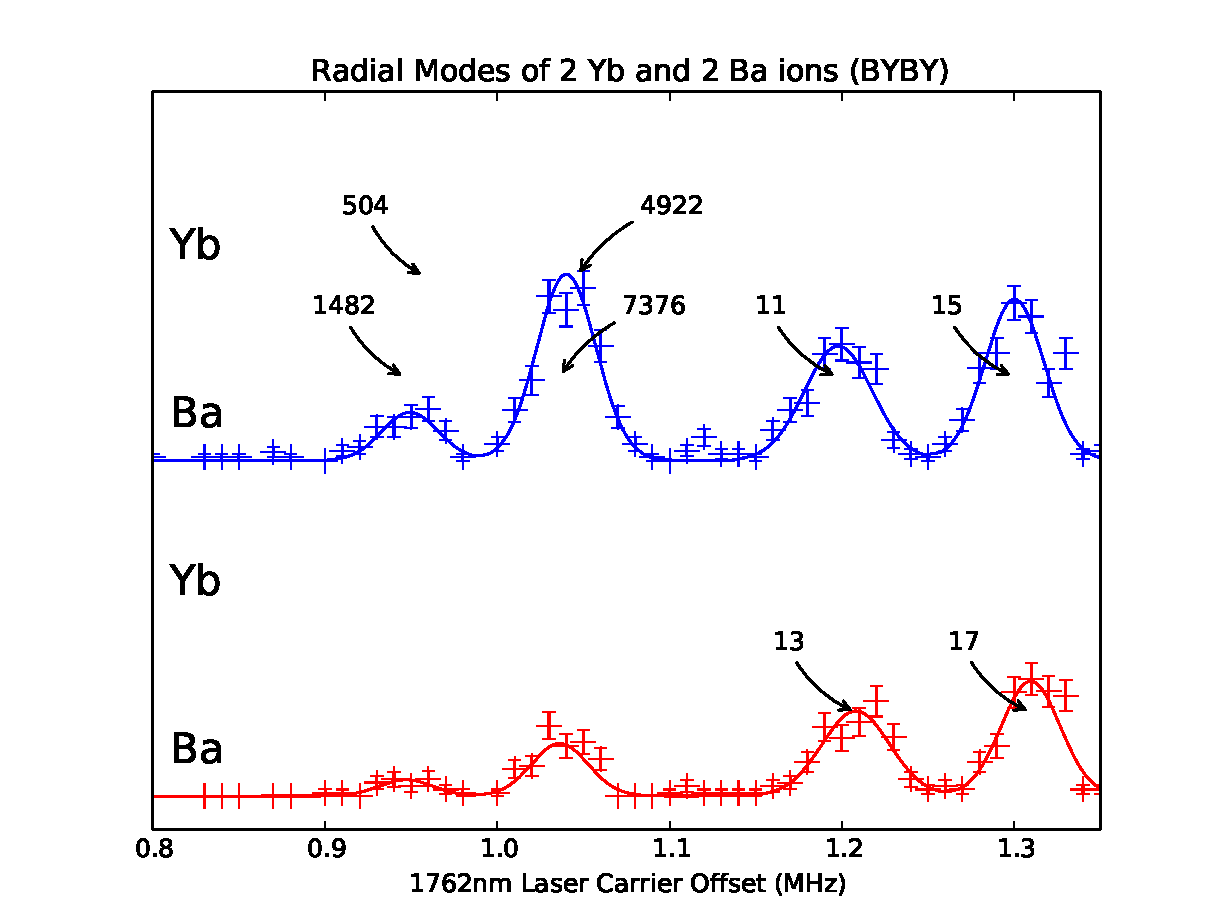
\includegraphics[width=0.7\textwidth]{RadialScanBYBY}
	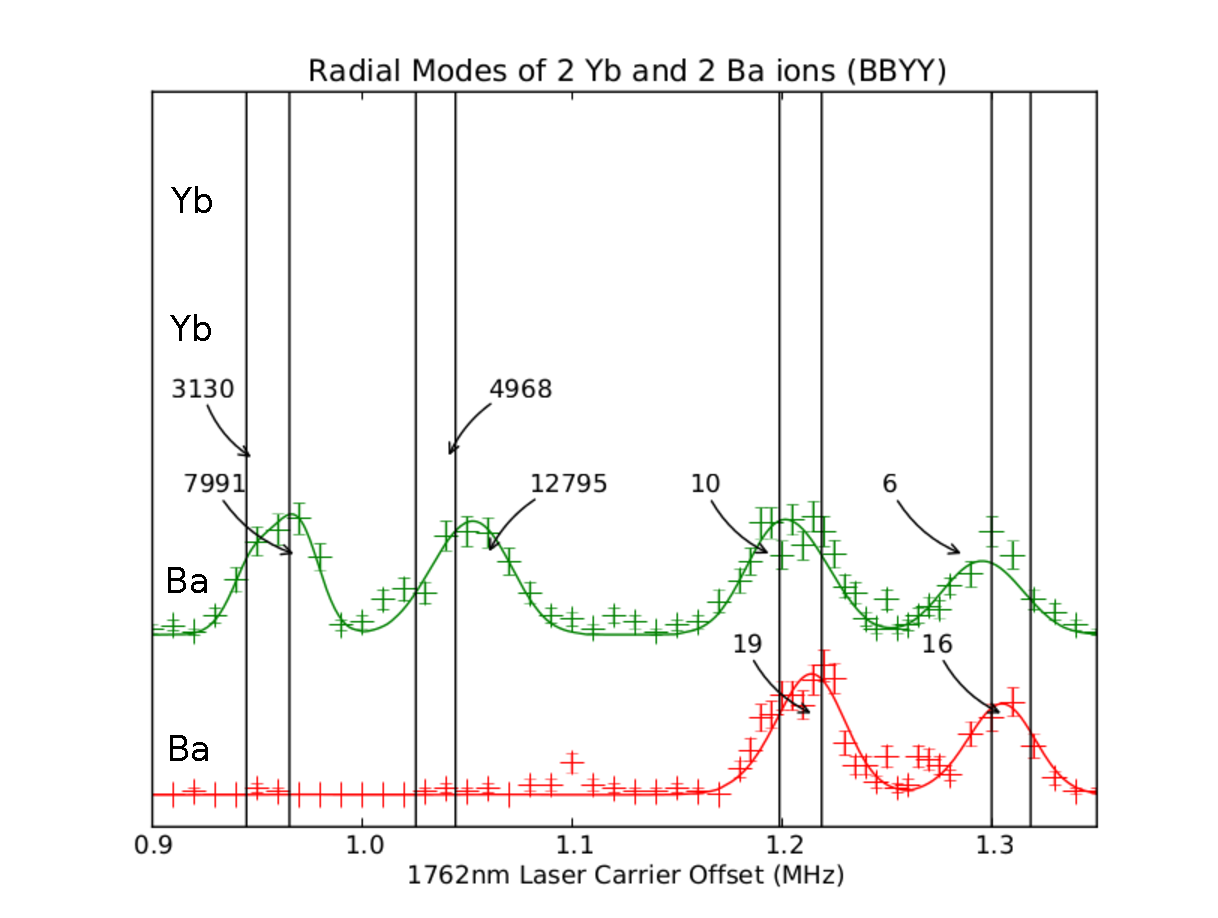
\includegraphics[width=0.7\textwidth]{RadialScanBBYY}
	\caption[Frequency scan over 1762~nm radial sidebands in a barium-ytterbium chain]{Frequency scan over the 1762~nm radial sidebands in a barium-ytterbium mixed species chain.  Predicted radial mode frequencies are shown by vertical lines while measured motional modes are labeled by arrows, along with their $\bar{n}$.  The vertical positions of the data curves show the locations of the barium ions in the chain with blank horizontal spaces representing the unaddressed ytterbium ions.  The top panel shows a Ba-Yb-Ba-Yb configuration and the bottom panel shows a Ba-Ba-Yb-Yb configuration.}
	\label{fig:radial-byby}
\end{figure}

After we have achieved the desired ion species configuration, we scan the frequency of the 1762~nm laser over the blue radial mode sidebands.  We limit the exposure time of the laser such that the shelving probability does not exceed 35\% allowing us to fit each peak to the weak excitation limit using Equation~\ref{eqn:shortpulses}.   In this limit, the shelving probability is given by
\begin{equation}
	P_\mathrm{shelve}(\omega) = \frac{1}{4} \eta_{\alpha, i}^2 \bar{n} \Omega_i^2 \frac{ \sin^2( (\omega - \omega_\alpha) t / 2) }{ (\omega - \omega_\alpha)^2 / 4 } \mathrm{,}
	\label{eqn:sidebands}
\end{equation}
where $\Omega_i$ is the Rabi frequency of the 1762~nm laser on ion $i$. In order to find $\Omega_i$ we also perform a Rabi experiment on the ion chain and determine the Rabi frequency for each ion by fitting to the resulting curve.  Again we have to deal with the frequency noise of the 1762~nm lock by allowing the 1762~nm frequency to vary over some range of frequencies.  Therefore, we actually fit the radial sideband curves to the integral of Equation~\ref{eqn:sidebands} over a Gaussian distribution of frequencies around a center frequency.  This frequency noise has the effect of broadening all of the radial modes and making it more difficult to fit the heights of modes close together in frequency.

The radial mode frequencies and eigenvectors are found from Equation~\ref{eqn:mixedtrap} following the numerical procedure described, but the measured radial mode frequencies display small, 10~kHz to 20~kHz, shifts from the theoretical frequencies.  We believe these shifts are due to small offsets in the error signal of the 1762~nm laser that occur when the laser is relocked.  The ZeroDer cavity that the laser is locked to also displays mechanical relaxation at a rate of 10~kHz/day, which explains some of the shifts because of the 10~hour experimental run time.  To accurately fit the peak heights we must also fit for the angular frequency of each mode, but the resulting frequencies are only shifted by 10~kHz to 20~kHz from the theoretical predictions.

First we will consider the case where the barium ions are maximally dispersed in the ion chain, i.e. the chain order is barium, ytterbium, barium, and ytterbium.  In top panel of Figure~\ref{fig:radial-byby}, a radial mode scan of this configuration is shown.  The two data curves are the probability of shelving the barium ion in that position as a function of the 1762~nm laser detuning.  The blank horizontal spaces correspond to the positions of ytterbium ions that are not addressed by any lasers.  The theoretically predicted radial modes given our independently measured trap secular frequencies are shown as black vertical lines.  The positions of the modes after the small frequency shifts are fit to them are indicated by the positions pointed to by the arrows, which label the fit $\bar{n}$ to each peak.  The four lowest frequency modes have large eigenvector motional components in ytterbium ions, but very small motional components for both barium ions.  It is clear from the labeled values of $\bar{n}$ that these modes are not being well cooled by the barium cooling lasers.  The mode frequencies, barium eigenvector components, and $\bar{n}$ for each mode in this configuration are given in Table~\ref{tab:byby}.  It is clear that there is a very large difference in the amount of motion that the last four modes have in barium ions than the first four.  We can also observe that having both eigenvector components be of the same magnitude does not decrease the number of quanta in the mode significantly, but even slightly increasing the maximum eigenvector component can have large effect.  Additionally, the participation of the barium ions in a given mode is increased when the base secular frequency for that direction is smaller.  

\begin{table}
\begin{tabularx}{1\textwidth}{ |>{\setlength\hsize{1\hsize}\centering}X|>{\setlength\hsize{1\hsize}\centering}X@{} >{\setlength\hsize{1\hsize}\centering}X|>{\setlength\hsize{1\hsize}\centering}X| }
	\multicolumn{4}{>{\centering\setlength\hsize{4\hsize} }X}{Ba, Yb, Ba, Yb Radial Mode Data} \tabularnewline
	Frequency (MHz) & 
	\multicolumn{2}{>{\centering\setlength\hsize{2\hsize} }X|}{ Barium Eigenvector Components } &
	$\bar{n}$ \tabularnewline
	\hline

	1.30 & 0.989 & 0.143 & 17 \tabularnewline
	1.29 & -0.144 & 0.989 & 15 \tabularnewline
	1.20 & 0.988 & 0.148 & 13 \tabularnewline
	1.19 & -0.150 & 0.987 & 11 \tabularnewline
	1.03 & 0.003 & 0.034 & 4913 \tabularnewline
	1.02 & 0.028 & 0.034 & 7427 \tabularnewline
	0.95 & 0.003 & 0.039 & 490 \tabularnewline
	0.94 & 0.033 & 0.041 & 1501 \tabularnewline
\end{tabularx}
\caption[Occupation number of modes in Ba-Yb-Ba-Yb chain]{Eigenvector components and occupation numbers for each mode in a chain of Ba-Yb-Ba-Yb ions.  The modes coupled strongly to ytterbium have much higher occupation numbers.}
\label{tab:byby}
\end{table}

When we move all of the barium ions to one side of the chain such that the order is barium, barium, ytterbium, ytterbium, we find the occupation numbers from Table~\ref{tab:bbyy}.  The temperature of the decoupled modes has increased substantially.  It is very clear from the eigenvector components of these modes and from Figure~\ref{fig:radial-byby} that the outermost barium ion is even more strongly decoupled.  It is fairly easy to conclude that for any reasonable chance of cooling all of these modes using barium ions, the barium ions will have to be interspersed along the length of the chain.  

\begin{table}
\begin{tabularx}{1\textwidth}{ |>{\setlength\hsize{1\hsize}\centering}X|>{\setlength\hsize{1\hsize}\centering}X@{} >{\setlength\hsize{1\hsize}\centering}X|>{\setlength\hsize{1\hsize}\centering}X| }
	\multicolumn{4}{>{\centering\setlength\hsize{4\hsize} }X}{Ba, Ba, Yb, Yb Radial Mode Data} \tabularnewline
	Frequency (MHz) & 
	\multicolumn{2}{>{\centering\setlength\hsize{2\hsize} }X|}{ Barium Eigenvector Components } &
	$\bar{n}$ \tabularnewline
	\hline

	1.31 & 0.866 & 0.500 & 16 \tabularnewline
	1.29 & -0.500 & 0.865 & 6 \tabularnewline
	1.20 & 0.865 & 0.501 & 19 \tabularnewline
	1.18 & -0.501 & 0.864 & 10  \tabularnewline
	1.03 & 0.002 & 0.022 & 12795 \tabularnewline
	1.01 & 0.002 & 0.029 & 4968 \tabularnewline
	0.95 & 0.002 & 0.026 & 7991 \tabularnewline
	0.93 & 0.002 & 0.035 & 3130 \tabularnewline
\end{tabularx}
\caption[Occupation number of modes in Ba-Ba-Yb-Yb chain]{Eigenvector components and occupation numbers for each mode in a chain of Ba-Ba-Yb-Yb ions.  The modes coupled strongly to ytterbium have much higher occupation numbers.}
\label{tab:bbyy}
\end{table}

In order to gain a simplified understanding of what this data tells us about the temperature of ions in mixed species ion chains, we have compared the $\bar{n}$ for each radial mode that is not cooled well by barium to its eigenvector components for barium ions.  The correlation between these variable seems to be strongest when we compare $\bar{n}$ to the maximum eigenvector component, $\max_{i,\mathrm{barium}} \left| \hat{e}_\alpha^i \right|$.  Plotting these variables against each other shows a strong correlation, with reasonable thermal occupation numbers only being reached when the eigenvector component is $\approx$ 0.04.

\begin{figure}
	\centering
	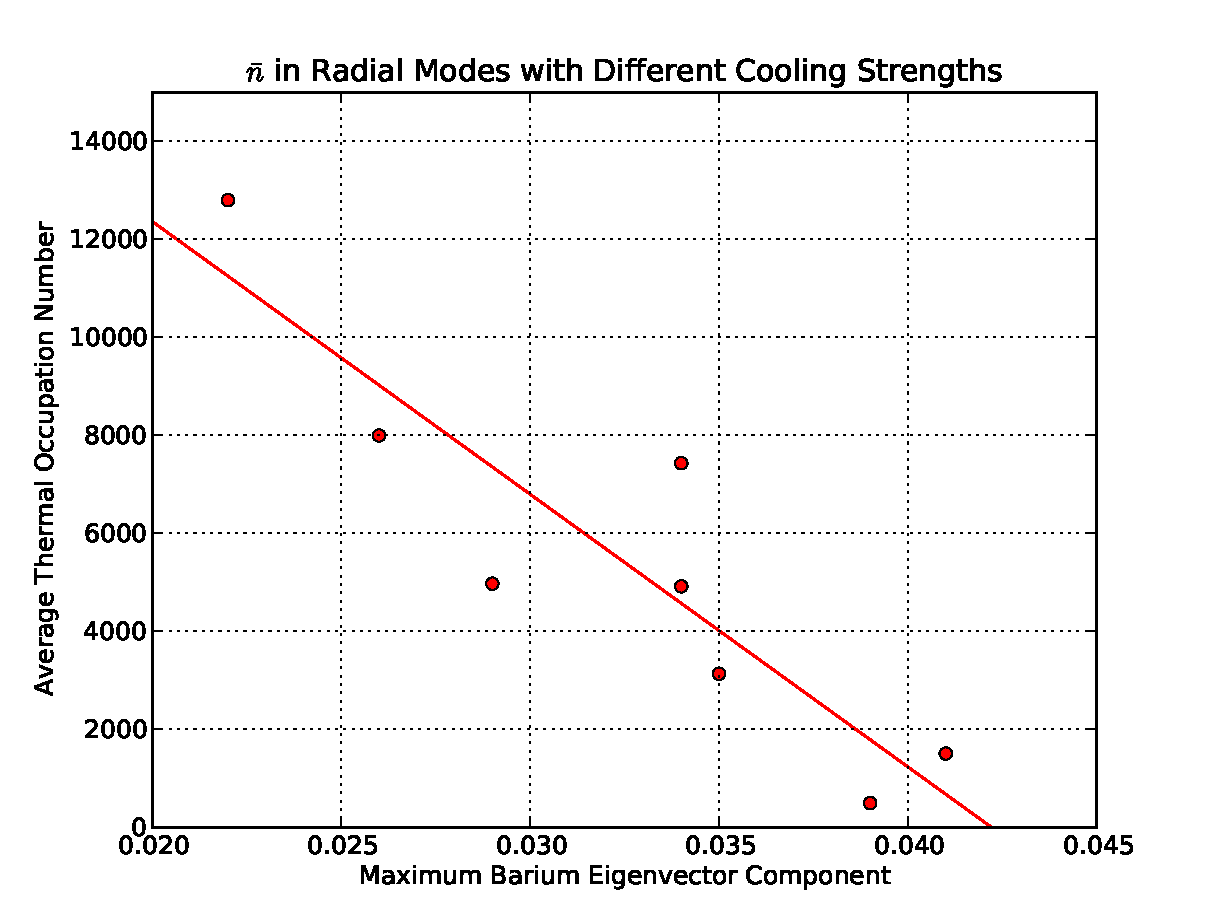
\includegraphics[width=0.8\textwidth]{RadialNBarEigenvectors}
	\caption[Radial mode occupation numbers for different barium ion motional couplings]{Radial $\bar{n}$ as a function of the maximum eigenvector component of the mode with a cooled barium.  The linear trend is given as a guide to the eye.}
	\label{radial-nbars}
\end{figure}

Obviously cooling ytterbium ions using only barium cooling lasers is not going to be as efficient as we would hope.  It seems that that our Doppler cooling is near optimal for barium ions, so it is unlikely that Doppler cooling alone will be able to perform any better than this.  There are still a few options for making progress however.  For the weaker of the two trap axes, we can see that the ytterbium modes are reasonably cold for chain configurations that are well mixed.  Only a few modes of the trap will need to be kept cold to perform entangling gates in ytterbium, and its possible the trap strengths and ion configuration can be arranged to make this possible.  Doing so will likely require the barium to be well distributed throughout the chain.

Investigating these problems for increasing numbers of ions should prove very interesting.  If the trends established above continue to hold it may still be possible to keep a few modes cold enough to be in the Lamb-Dicke regime and perform entangling operations in ytterbium.  Working with more ions will most likely involve moving this experiment to a surface electrode trap where the ordering of the ions can be easily controlled.  Scaling this experiment further in its current trap would be very difficult.

\section{Ion Species Reordering}
\label{sec:reordering}

Working with mixed ion species chains gives an experimenter the ability to determine when chains reorder.  Obviously when working with only a single ion species, the ions are indistinguishable and it is impossible to tell whether its order is the same as previously at any point in time.  We hypothesized that the reordering of ions would happen at a relatively constant temperature and therefore could provide a simple temperature or heating rate measurement.  To investigate this hypothesis we performed simulations of the motion of mixed ion species chains.

Heating in ion chains is difficult to simulate well because it often depends on random electric field noise which is difficult to integrate numerically.  Instead of simulating the heating process, the ions are initialized at the beginning of the simulation to a given temperature.  Depending on this initial temperature, we track the probability for them to reorder before they are cooled to somewhere near their ground state.  The initial temperature is modeled by initializing the ions velocity to the corresponding energy with a random direction.  The ions motion is then modeled subject to the differential equation
\begin{equation}
	m_i \ddot{\vec{x}}_i = \vec{F}_\mathrm{trap}(m_i) + \hbar \vec{k} \frac{\Gamma}{2} \frac{s}{1 + s + 4 \left( \frac{\delta + \vec{k} \cdot \dot{\vec{x}}}{\Gamma} \right)^2}	+ \sum\limits_{j \ne i} \frac{1}{4 \pi \epsilon_0} \frac{e^2}{ \left| \vec{x}_i - \vec{x}_j \right| ^3 } \left( \vec{x}_i - \vec{x}_j \right) \mathrm{,}
\end{equation}
where $\vec{x}_i$ is the position of the ion that began in position $i$, $\vec{F}_\mathrm{trap}$ is the harmonic trapping force that confine the ions, and $s$, $\Gamma$, $\delta$, and $\vec{k}$ are the saturation parameter, natural linewidth, detuning, and wavevector of the main Doppler cooling laser.  This differential equation is numerically integrated using the Boost odeint library\footnote{\url{http://www.boost.org/doc/libs/1_57_0/libs/numeric/odeint/doc/html/index.html}}.  Once the ions reach a sufficiently low energy, it is determined whether the ion species have reordered in a way that is experimentally detectable.  Figure~\ref{fig:reorderingpos} shows a sampling of the axial positions of a chain of ions from a single run of the simulation where the ions reorder.  Repeating this process several thousand times for several initial temperatures shows us that the probability to reorder changes relatively sharply with temperature.  Using a single quad-core desktop the runtime for performing 10,000 iterations of this procedure is almost a day because of the difficulty of integrating singular potentials and the long integration times used.

\begin{figure}
	\centering
	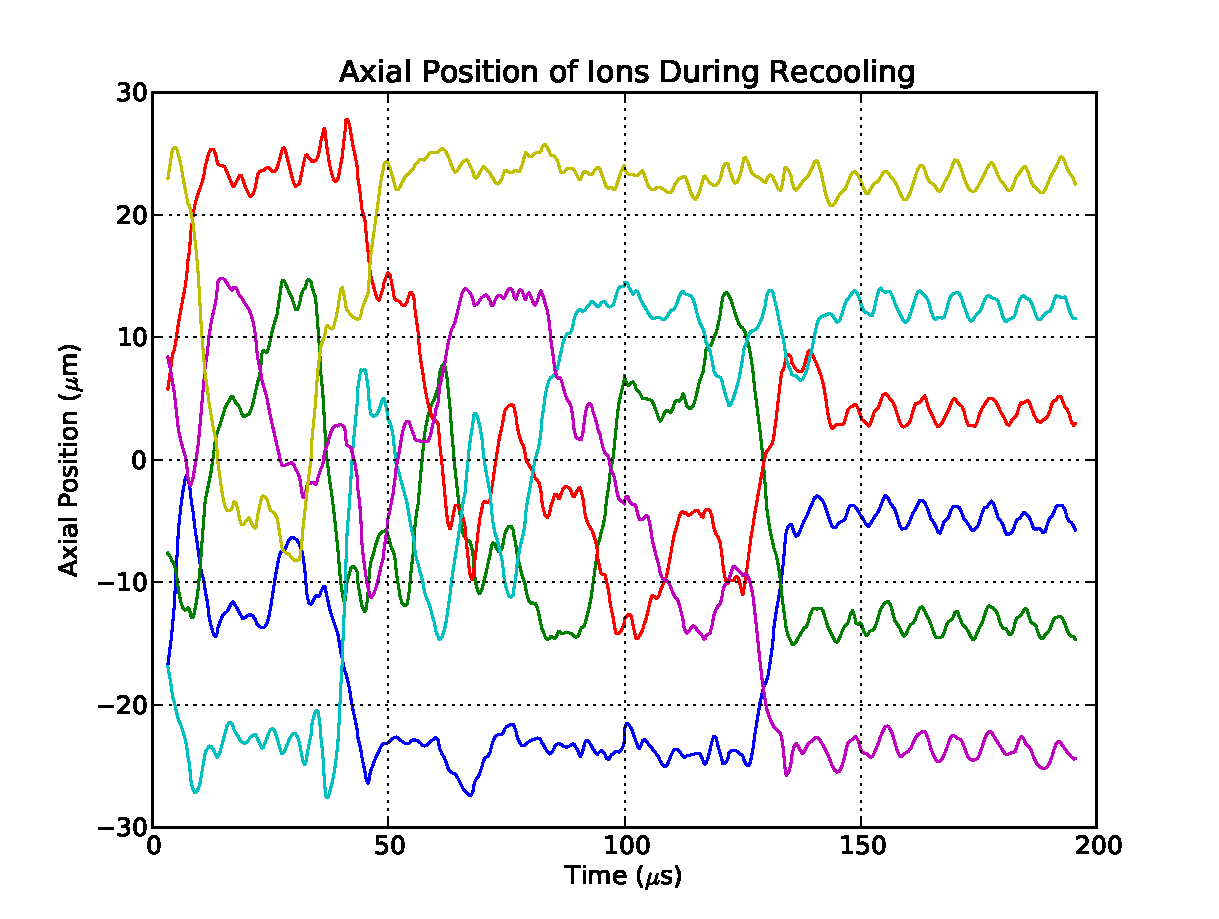
\includegraphics[width=0.8\textwidth]{ReorderingPositions}
	\caption[Simulated axial positions during Doppler recooling]{Simulated axial positions of trapped ions as function of time.  The ions are initialized with a large randomly directed velocity and are cooled by simulated Doppler cooling.  The numerical integration is performed by the odeint library.}
	\label{fig:reorderingpos}
\end{figure}

\begin{figure}
	\centering
	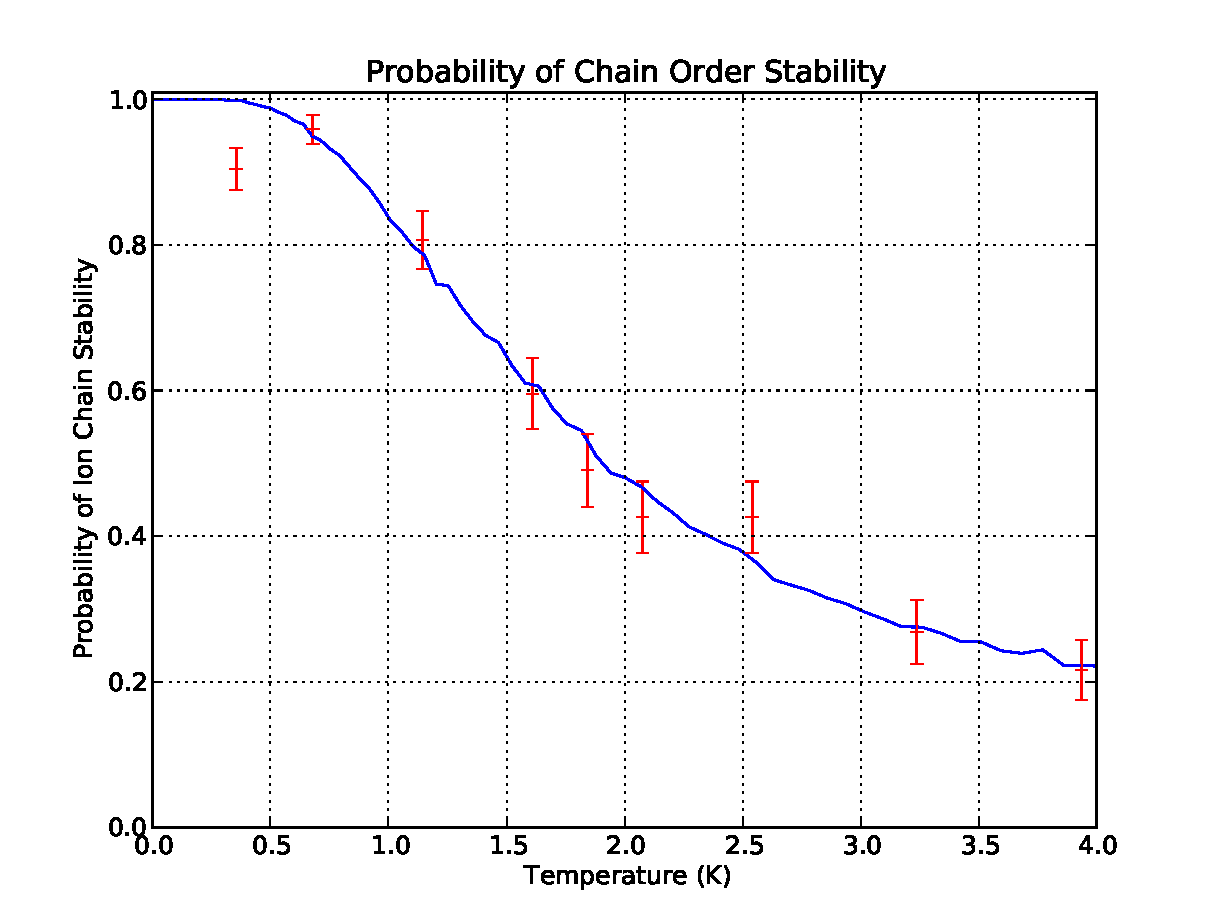
\includegraphics[width=0.7\textwidth]{Reordering81}
	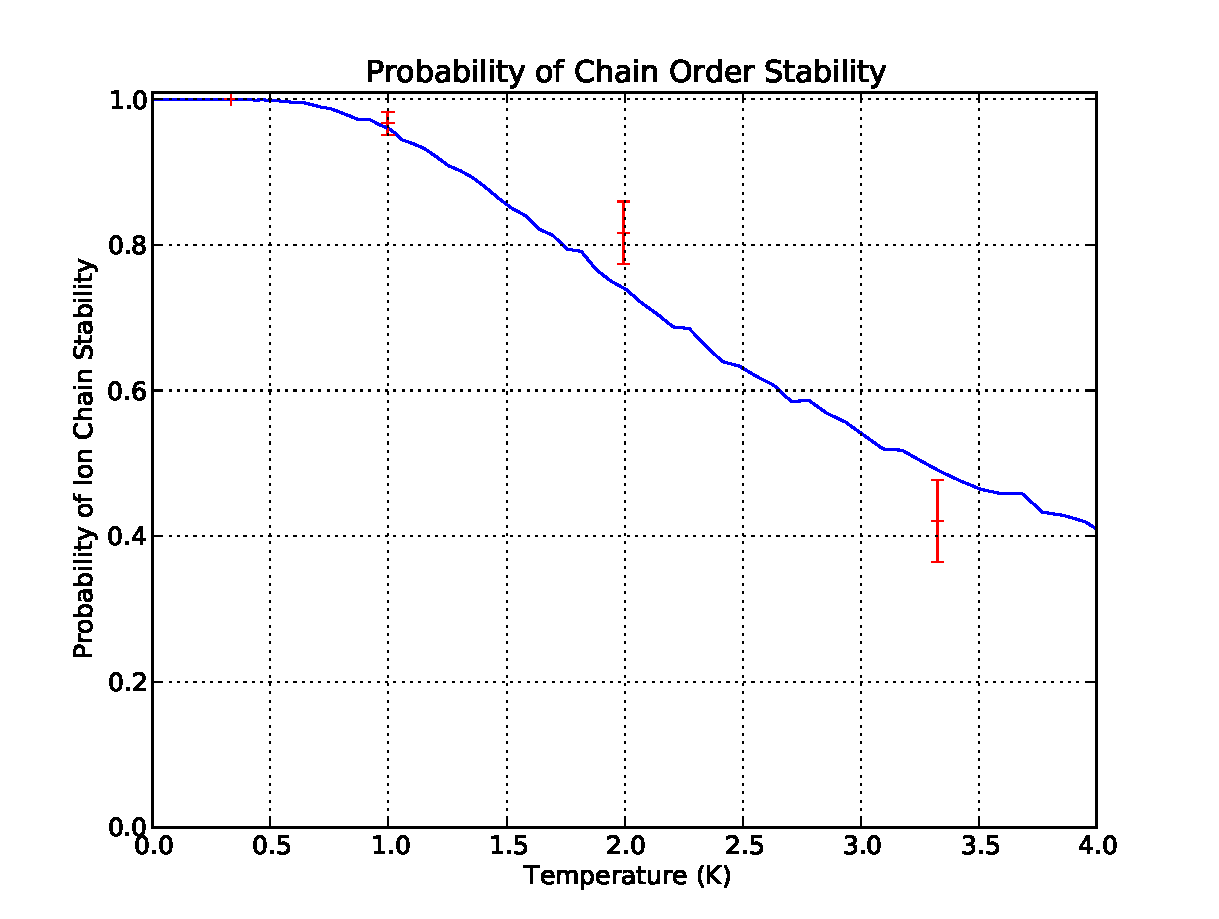
\includegraphics[width=0.7\textwidth]{Reordering61}
	\caption[Reordering probability of ion chains at different temperatures]{Reordering probability as a function of temperature.  The simulation results are shown in blue, while the red data points are taken at different uncooled times and then fit to temperatures using a linear heating rate.  For seven barium and one ytterbium ion (top) the initial temperature is 0.215~degrees Kelvin and the heating rate is 0.465~K/s.  For five barium and one ytterbium (bottom) the initial temperature is 0~K and the heating rate is 0.665~K/s.}
	\label{fig:reordering81}
\end{figure}

Experimentally, ion species reordering probabilities are very easy to measure.  Once again heating can be induced by allowing the ion to spend several hundred milliseconds to several seconds uncooled in the trap.  Using our EMCCD camera we image the ions before and after a given period of uncooled time.  The reordering probability is then extracted from a series of many such experiments.  In order to fit the collected data to the theoretical curve generated by the molecular dynamics simulation, we need to fit the initial temperature and heating rate of the ion chain.  

In Figure~\ref{fig:reordering81}, the resulting curves for an ion chain of 7 barium and one ytterbium ion are shown.  The fit indicates an initial temperature of 0.215~degrees Kelvin and a heating rate of 0.465~K/s.  For five barium ions and one ytterbium ion the initial temperature is 0~K and the heating rate is 0.665~K/s.  Obviously, this initial temperature is not physically realistic and is probably caused by the small amount of data taken using the smaller chain.  More data would have had to be taken to fit a reasonable initial temperature because its effect on the fit is relatively small.  The heating rate measurement should be reliable because it has a strong effect on the generated points.  A heating rate of 0.465~K/s corresponds to 8.07~quanta/ms for 1.2~MHz phonons.  This rate is 2.8 times larger than the radial mode heating rate of 2.84~quanta/ms for a single barium ion measured using Rabi flop decay, but it also includes the motional energy in the axial motional modes.  We have not directly measured the heating rate of these modes, but this total heating result seems reasonable because their heating rate is expected to be larger because of their lower frequency.

The advantage of this technique is that a single, fast measurement can quickly characterize the heating rate of the trap.  With the methods described earlier in this chapter several dozen data points each comprised of several hundred experimental runs must be performed to fit a function and determine the ions' temperature or heating rate.  Also, the configuration of the ion species must be controlled in order to analyze the same motional mode structure.  With the present method, collecting one or two data points near the maximum slope of the reordering probability can generate a quick measurement of the same quantity and, obviously, no effort to control the species configuration is necessary.  The reordering measurement also does not require any narrow transitions to be used, allowing traps to be quickly be characterized even before these additional lasers are aligned to them.

\begin{figure}
	\centering
	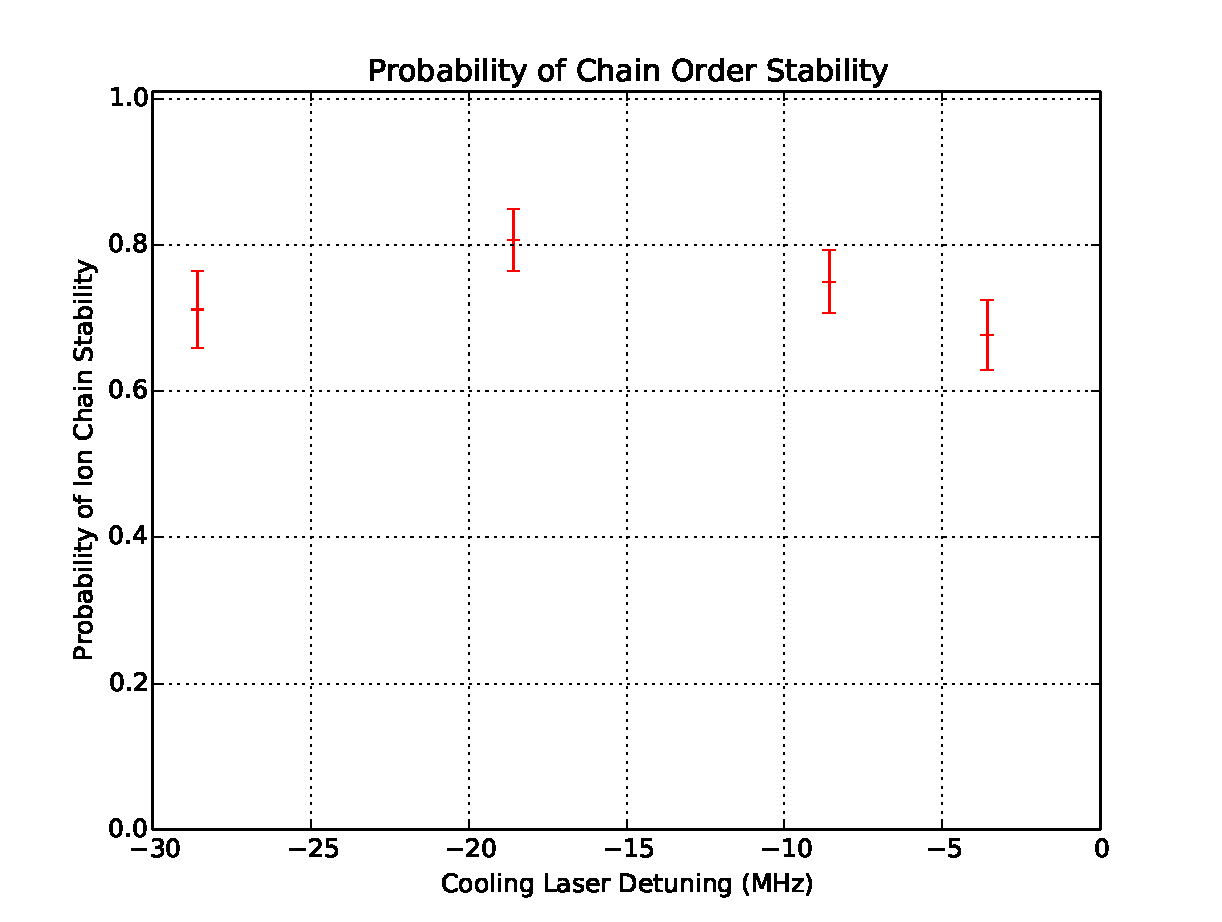
\includegraphics[width=0.8\textwidth]{ReorderingFreq}
	\caption[Reordering probability at different cooling laser detunings]{Reordering probability of a linear chain at different Doppler cooling laser frequencies.  The ions are allowed to heat for 2~seconds before the reordering is detected so that the rate of change of the reordering probability as a function of temperature is maximized. Lower probability of chain stability indicates lower cooling efficiency.  Although the variations are small, the results could be made statistically significant by taking more data.}
	\label{fig:reordering-freq}
\end{figure}

Since these measurements are so quick to carry out, it is also convenient to look at how our minimum temperature varies with our 493~nm laser frequency using this technique.  Figure~\ref{fig:reordering-freq} plots the reordering probability as a function of the detuning of this main barium cooling laser with the uncooled time in the experiment set to the maximal reordering slope.  Collecting data using this method took only a few minutes as compared to an hour or more to measure several curves with the other methods described.  For this reason, reordering measurements also serve as a good, fast indicator of cooling efficacy.  Although we saw earlier that this technique is not always a good measurement of initial temperature, when sitting on this maximal slope we can definitely see the effects of the Doppler cooling parameters.

In this chapter we have characterized the temperature and heating rate of barium and ytterbium ions in our trap in many different ways.  The benefit we were hoping to achieve in designing this system was the ability to continuously cool barium ions while performing quantum operations with ytterbium ions.  It certainly looks like that task is not going to be as easy as we had hoped.  In Chapter~\ref{sec:qcomp}, we found that we needed to be operating in the Lamb-Dicke regime where $\eta^2 \bar{n} \ll 1$ in order for M\o{}lmer-S\o{}rensen entangling operations to have high fidelity.  At the current average thermal occupation number of some of the modes and the expected $\eta$ for our laser we can expect $\eta^2 \bar{n} \approx 1$.  We are hopeful that by manipulating additional trap parameters in surface traps and using additional barium ions we can lower these temperatures, but if necessary we can also perform these entangling gates using the better coupled axial modes.  There are still many different possible degrees of freedom to explore in this new system.

